\chapter{Introduction}

Reconstructing the human connectome at the neuron-level is a daunting task. It would take a trained neuroscientist roughly 400 trillion hours to manually reconstruct the 3D-geometry of an entire human brain from cell-level electron microscopy images of brain tissue\footnote{This is a rough lower-bound estimation, assuming that that it takes a neuroscientist roughly one hour to reconstruct the geometry of a $6\mu m \times 6\mu m \times 200nm $ section of tissue and that the average human brain has a volume of $1300\mathsf{cm}^{3}$.}. Considering that the universe has only existed for roughly 112 trillion hours, it is unlikely that humans will ever manually reconstruct the entire human connectome. And yet, knowing the entire neuron-level human connectome would be eminently useful across the field of neuroscience. We can do better - not with humans, but with machines.


\section{Overview of Contributions}

This thesis is an exploration into various automated methods of reconstructing the 3D geometry of neural tissue through image segmentation. Specifically, we attempt to increase the performance of existing automatic EM segmentation pipelines, both in efficiency and accuracy, by exploring modifications at various stages of these pipelines. 

Throughout our initial exploration of existing EM segmentation methods, it became increasingly clear that, since the output of one stage of the segmentation pipeline feeds directly into the next, errors at any given stage will inevitably propagate to later stages. There are generally two approaches to mitigating this propogation effect: reduce the errors introduced at any given stage (i.e. increase the accuracy of an intermittent neural net), or make subsequent stages more robust to errors in previous stages (i.e. add substantial augmentations to training, apply techniques like Mean Affinity Agglomeration to segmentations). This thesis touches on both types categories of improvement.

While this thesis research was conducted in conjunction with several other undergraduates, graduate students, and a professor in the Princeton Neuroscience Institute, this thesis will detail my individual contribution. Specifically, my contribution can be broken up into three parts:

\begin{itemize}
\item The creation of the \texttt{DeepSeg} segmentation pipeline, a modular framework written in Python that allows for easy training and prediction with current popular models, as well as easy experimentation at different stages in the computational pipeline.
\item Experimention with several different architectures for transforming raw segmentation images into affinity/boundary maps, attempting to improve overall accuracy and noting their invariance to errors in earlier stages of the pipeline.
\item Exploration of learned alignment strategies, both on learned transformations and in an end-to-end setting.
\end{itemize}

\section{Motivation}

In the field of computational neuroscience, there exist a class of problems relating to mapping the neuron-level structure of the brain. For instance, one might want to precisely model the neural connectivity of an abnormal mouse brain, or observe the connectivity and topology of a worm at different stages of its development. Conventionally, the structure of the brain is inferred from images, whether they are thin slices of a brain imaged with an electron microscope, volumetric images acquired using digital radiograhpy systems (i.e. fMRI, CAT, etc), or visible-spectrum video of exposed brain tissue. Although these imaging technique generate information at different resolution levels, they invariably present a huge data problem: when researchers are presented with small-scale image data, it is fundamentally infeasible to efficiently infer the connectivity and structure of a small cluster of neurons by hand, let alone an entire brain or nervous system, simply because the amount of neurons in a brain is too large.

Many attempts have been made to automate the process of inferring connectivity and topology from images using various algorithmic and machine learning models. In the past five years or so, many of the most successful attempts at this class of problems have utilized Convolutional Neural Networks (CNNs) to achieve their high performance. The goal of this year-long project is to explore many of the different CNN-based approaches that have gained recognition in the past few years in several sub-problems, evaluate their performance and enumerate their deficiencies, and attempt to design new architectures that achieve improved performance in these sub-problems. In addition to increasing performance on established benchmarks, we also make contributions on new sub-problems for which there are no established benchmarks.

The motivation for the research in this field is to better understand the connectivity of neural tissue. Since this is such a broad goal, it stands to reason that there a number of intermediary sub-problems that can be tackled to learn about connectivity. Several of the sub-problems have been heavily studied, and various public competitions have been organized that provide labeled training data and unlabled test data, encouraging competitors to achieve maximum performance against a certain benchmark. As we developed our models, we submitted their predictions to several of these open competitions, often performing well.

\section{Related Work}

\TODO{Flesh out more background on CNNs}
\TODO{Semantic Segmentation}

\subsection{Connectomics}

\subsection{Image Segmentation}

\subsection{EM Segmentation}

\TODO{VD2D, VD2D-3D}
\TODO{N4}
\TODO{Res Net}
\TODO{Segnet}
\TODO{}

\subsection{Alignment}

The problem of determining the connectivity of a brain falls in the sub-field of connectomics, which has been a lively area for research for over 30 years. The first full connectome of an organism was created in 1986, producing the mapping of the brain of \textit{C. elegans} \cite{White1986}. Since then, partial and full topological and connectivity maps have been created on various organism, often using electron microscopy and careful hand-reconstruction to do so. More recently, by genetically modifying organisms to produce proteins that become phosphorescent in the presence of calcium (calcium is released across the synapse between a dendrite and an axon when a neuron is fires), researchers have been able to monitor both brain activity and neural structure using video photography in the visible spectrum \cite{Nguyen2015}.

In terms of the computational approaches to automating connectome reconstruction, many groups have attempted to create systems to accomplish near-human accuracy when labelling neurons in the brain. In the early 2010's, a group of researchers published an open dataset and created a global challenge to use machine learning methods to label neurons in image slices of a brain, resulting in the creation of models with near-human accuracy \cite{Arganda-Carreras2015}. More recently, researchers at Princeton University applied similar approaches to automatically detecting neurons in videos formed with the calcium imaging techniques mentioned above \cite{Apthorpe2016}.

The work in the field continues to improve mapping techniques, but our understanding of learning methods in both computational neuroscience and computer vision are in their infancy, and are not yet practical for deployment on a larger organism (i.e. a human) due to computational and accuracy issues. This project hopes to improve on existing methods, even if incrementally, so that we can better understand what an efficient mapping approach capable of mapping a full brain might look like.

\section{EM Segmentation Pipeline}

So far, we have referenced "EM Segmentation Pipeline" as a process that converts raw EM images into 3-dimensional segmentations of the structures those images represent. There are several computational stages of this pipeline, and in order to understand how altering the pipeline will affect overall performance it is necessary to explain in detail the various components of this pipeline. While different segmentation techniques may use some subset or superset, the pipeline I outline below is a general conceptual representation of what most state-of-the-art segmentation schemes utilize. 

The EM Segmentation Pipeline can roughly be separated into five components, shown visually in Figure \ref{fig:segmentation_pipeline}:

\begin{figure}
\centering
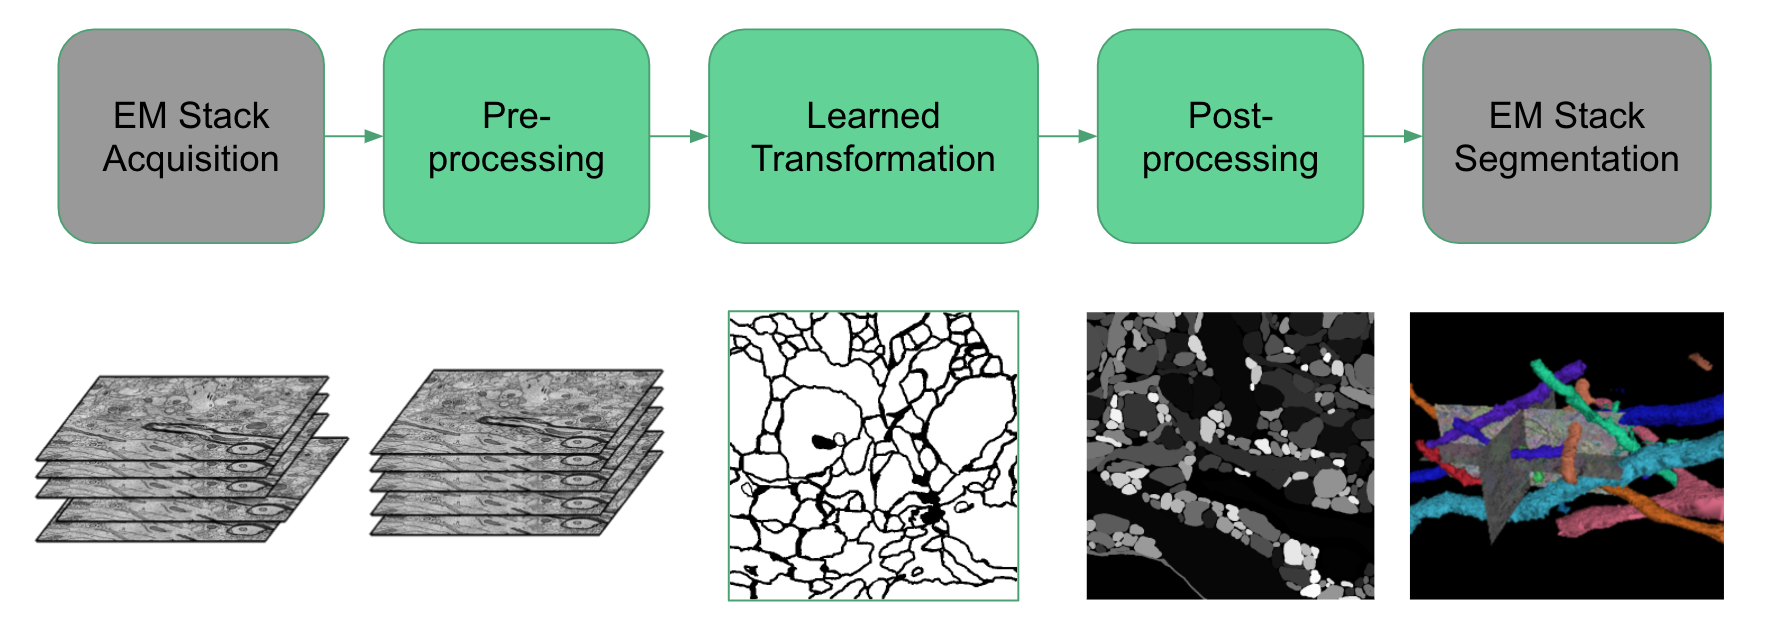
\includegraphics[width=\textwidth]{img/seg_pipeline.png}
\caption[A general outline of the EM segmentation pipeline]{A general outline of the EM segmentation pipeline. The lower set of images represent intermediate stages that the data takes on during processing. In this example, the images are first acquired through some sort of electron microscopy technique (typically ssTEM). Second, they undergo preprocessing, which is primarily realignment of slices that were disrupted in the imaging process. Third, a learned transform is applied, which in this case transforms the stack of images into an affinity map. Fourth, postprocessing is applied, which in this stage is computing an actual segmentation from the predicted affinities. Fifth, geometric segmentation is inferred from the pixel segmentation, and the data is ready for use in a downstream task. }
\label{fig:segmentation_pipeline}
\end{figure}

\subsection{Image Acquisition}
Given a physical volume of neural tissue, the first task in inferring tissue structure is to acquire some sort of digital representation of this tissue. While there are many techniques available for imaging biological tissue (e.g. light microscopy, electron microscopy, radiography, magnetic resonance imaging), typically the only way to acquire a representation of cell-level structures is by using a tunnelling electron microscope (TEM). \TODO{Find a citation for this} Before imaging, samples undergo considerable preparation: typically, they are embedded in a rigid medium that will allow them to be sliced with minimal distortion; additionally some sort of stain is applied to the tissue that affects the electrical properties of different biological structures, allowing for high-contrast imaging. The result is a set of slices of neural tissue, 30-50nm thick, that can be independently imaged in the SEM. When positional order from slicing is combined with the raw image data (which takes the form of grey-scale images, as opposed to RGB or CMYK images), each individual value can be treated as a voxel, since it is indexed by three orthogonal coordinates. Important to note is that these voxels are anisotropic, meaning that they are larger in the z-dimension than they are in the x-y dimension. This introduces a computational complexity that can somewhat be compensated for at later stages of the pipeline.

Although the actual performance of this physical imaging process is far ouside the scope of this thesis, we mention the physical steps involved because the methods used in preparing and imaging biological slices have immediate consequences on the quality of the data that is fed into stages of the pipeline in which we are primarily interested. Because the imaging process is physical and involves structures at nano-scale, physical preparation of the sample can introduce various defects into the slices that show up in resulting images. The staining process, for instance, can inconsistently vary contrast throughout an image, and can produce large dark blotches in an image. The slicing procedure can create tears and folds in tissue, which manifest as discontinuities in the images, and can even physically translate slices hundreds of nanometers. And since neural tissue naturally contains significant quantities of water, samples are prone to dry inconsistently, resulting in elastic warping of cell-level structures (like a rubber sheet that has local stretching). Visual examples of some of these artifacts can be found in Figure \ref{fig:imaging_errors}

\begin{figure}
\centering
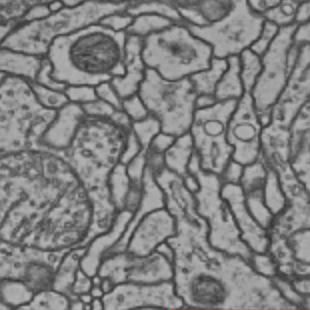
\includegraphics[width=0.3\textwidth]{img/normal_example.png}
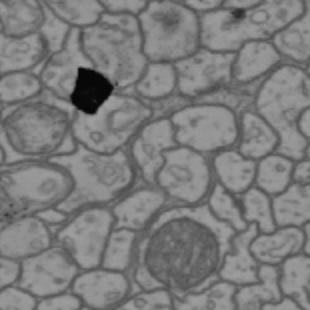
\includegraphics[width=0.3\textwidth]{img/stain_error.png}
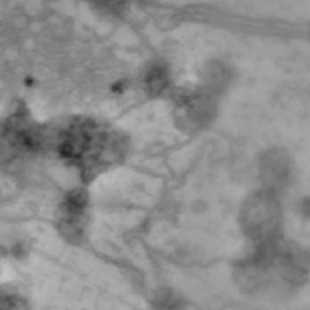
\includegraphics[width=0.3\textwidth]{img/blurred_example.png}
\caption[Examples of defects in the imaging process.]{Examples of defects in the imaging process. Left: a properly stained and imaged segment. Center: a slice where inconsistent staining or another artifact has left a large dark spot on the image. Right: a slice that was prepared in such a way that the microscope couldn't produce a sharp image, either during slicing or focusing.}
\label{fig:imaging_errors}
\end{figure}

These deformations caused by the imaging process can have drastic implications in the performance of later stages of the pipeline, especially when those stages aren't explicitly corrected for. We noticed that even slight misalignments in image data caused ultimate segmentation performance to noticably suffer. Later in the pipeline we will explore various techniques that can be used to make the pipeline more robust to these inevitable imaging defects.

\subsection{Preprocessing}
Once volume data is acquired, data usually will undergo any of several preprocessing techniques to prepare it for later stages of the pipeline. The scope of preprocessing and types of data transformations performed vary depending on the robustness of later stages of the pipeline, as well as requirements on the output of the segmentation pipeline. Preprocessing is generally trated as distinct from subsequent stages of the pipeline because the transformations often keep the data in the same domain of values, and maintain the data representation. In other words, both the input and the output of preprocessing take the form of stacked EM images. Typically, preprocessing will include some form of image adjustment and stack realignment.

Image adjustment can be as simple as altering the contrast on individual images, or making contrast uniform across the entire stack. While these adjustments will typically improve segmentation results, most modern deep learning techniques (which are liberally used in the subsequent pipeline stage) are easily trained to be quite robust with respect to level differences betweein images, so a rigorous exploration of image adjustment techniques would likely yield marginal gains in accuracy.\footnote{Training speed, however, could potentially see significant improvements, as a neural net would have to learn fewer functions if input were more uniform} 

The same cannot be said for image alignment. The defects and imprecisions introduced in the actual imaging process can severly impact segmentation performance, particularly because they introduce three-dimensional discontinuities that make it difficult for many neural networks to trace continuous segments across slices. Thus, automatic stack alignment is an active area of research.

At its heart, the alignment problem is one of misrepresentative data. Ideally we would like each 'voxel' to spatially correspond to a true volume in the sample, and for a voxel's position in the the data to correspond to its true position within the greater sample. The defects in the imaging process taint this mapping, and we are left with a dataset that, when taken literally, misrepresents the physical volume from which it was derived. Thus, the task of realignment is to take this noisy data and distort it in some way so that it more accurately corresponds to the original volume.

While there are many theoretical ways of registering two images (registration here means alignment and distortion so that their features align accurately), most modern methods rely on establishing points of correspondence between two or more images, and distoring the images such that those points of correspondence end up at the same x-y coordinate in all images. It is generally believed that, given a high enough density of true correspondences throughout a stack, one can transform the data into a form that is pixel for pixel true to the actual cellular structure of a sample.\footnote{Intuitively, this makes sense, since structures within cells are physically connected, our notion of correspondence is essentially a description of how these structures are physically connected.} The transformations themselves can be parameterized as elastic transforms, which provide discrete interpolation for all voxels not labeled as correspondences.

The problem, then, lies in actually determining these correspondences with high accuracy and high enough density for sample-accurate registration. One popular tool for achieving rough correspondences is \texttt{TrakEM2}, which provides functionality for registering generic images using a combination of the Scale Invariant Feature Transform (SIFT) and a global optimization algorithm. This algorithm uses no learned or otherwise domain-specific knowledge, and is widely used across computer vision applications to stitch arbitrary images together. This process is sufficient for establishing rough correspondences, but the noisy and varied nature of cellular structures means that, without any more domain-specific correspondence labeling the resulting image registration on a moderately distorted dataset will likely not result in transformations that are smooth or accurate.

The Seung Lab's current realignment techniques attempt to use domain-specific techniques to achieve correspondence. These techniques are typically hand-designed filters that draw on domain knowledge of the consitution of EM slices of neural tissue, and require a non-trivial amount of hand-tuning when applied. To compute a realignment, first a sparse set of correspondences are made at the macro level, and a rough realignment is iterateively computed (the rationale being that iteratively computing many fine realignments has slow convergence and is computationally unfeasable). Following this rough realignment, a much more granular set of correspondences are computed, and the stack is iteratively deformed a small number of times to compute a smooth, converged registration. This technique is quite effective, and leads to near-perfect registration, but requires a substantial amount of trained human input to determine both the parameters for the various correspondence filters and to correct obviously incorrect correspondences.

A more desirable approach would be to use machine learning to train a large set of filters (more specific ones than humans could compute) to predict correspondence at different levels of granularity. This is an active area of research within the Seung Lab. Alternatively, machine learning could be used to learn the actual parameters for a piecewise affine or elastic transform, rather than learn filters to predict corresponence, although as we demonstrate in Chapter 5 this is potentially quite difficult. 

Again, it is worth noting that failures in preprocessing to compensate for errors in the imaging stage - as well as new artifacts introduced in the preprocessing stage - will be propagated through the remainder of the pipeline, and can only have a negative or neutral impact on segmentation performance.

\subsection{Image Transformation}
The image transformation stage of the segmentation pipeline can loosely be defined as any set of transformations that compute a representation of the sample that is different in kind from a set of aligned images. In the case of most of the models discussed in this paper, the image transformation stage converts a stack of EM images into a 3D pixel-wise affinity map, where the labels at each pixel represent the probability that that pixel is in the same cellular body as the adjacent pixel in the x, y, and z direction. For other segmentation schemes, like Google's Flood-Filling architecture, the transformation output is a direct segmentation. 

This stage is perhaps the most well-explored in the pipeline for neural segmentation. While in the past hand-crafted or generic techniques were used in this stage to some degree of success (i.e. selective thresholding, hand-crafted filters, etc), most state-of-the-art techniques utilize some sort of machine learning scheme to learn the output representation, usually a neural net architecture that utilizes many successive convolutions to predict each pixel (or a small patch) of the output segmentation. These pixel/patch predictions can be stitched together to make a prediction on a whole stack. These ML approaches are typically supervised, and rely on using large datasets annotated with segmentations for training. Thus, as in most deep learning applications, the size and diversity of the training set is one of the most important factors in maximizing the generalization performance of this stage of the pipeline.

Because large, high-quality, labeled EM datasets are hard to come by (see the second sentence of this thesis), most researchers will take a reasonably-sized dataset and randomly apply data augmentations that make the data look like fresh data, thus artificially expanding the size of the dataset. These augmentation techniqes can broadly categorized as either affine transforms or elastic transforms. Specifically, researcher will usually introduce som sort of scaling, rotation, shearing, and elastic warping to both the image stack and the labels. These techniques have an enormous impact on accuracy and generalization - empirical evidence of this will be provided in Chapter 3.

The specific network architectures that are used in this stage of the pipeline are quite varied. We will describe the general classes of architectures relevant to our exploration here, and will revisit specific architectures we used later in this paper. Additionally, it is worth noting that elements of various architectures listed below can be combined (i.e. adding residual connections to standard convolutional nets.)

\subsubsection{Standard Convolutional Networks}

\begin{figure}
\centering
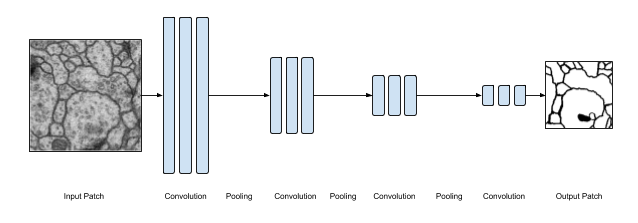
\includegraphics[width=\textwidth]{img/Fully_Convolutional_Network.png}
\caption[A prototypical Fully Convolutional Neural Network]{A prototypical Fully Convolutional Network, with successive convolutional layers followed by pooling layers. Depending on the types of convolution layers, the size of the input may be much larger than the size of the output, implying that the field of view for each pixel in the output could be greater than 1.}
\label{fig:fully_conv_net}
\end{figure}

The most conceptually simple type of network that is used is the standard convolutional network, depicted in Figure \ref{fig:fully_conv_net}. Standard convolutional nets typically involve several successive convolutions with small filters (e.g 3x3x3 filters) that perform either 'valid' or 'same' convolutions.\footnote{See Appendix B for more details about convolution.} After each convolution, a nonlinearity (e.g. ReLU) is applied, and every so often pooling layers are interspersed to alter the scale of the underlying feature maps. At the end of these alternating convolutions and poolings is a prediction, often the output of a sigmoid, that predicts a single pixel or patch of boundaries (or affinities, in the 3D case). Depending on the number of convolutions and poolings, the output pixel is determined by pixels within a certain field of view in the input image - that is, if one were to mathematically unrool the convolutions and poolings, only a certain number of pixels in the input image would be used to compute the prediction in the output image. In the N4 architecture applied in 2 dimensions, for instance, each pixel in the output prediction is influenced by pixels in a bounding box of 96x96 pixels. Architectures that are primarily Standard Convolutional Networks include N4 (2-dimensional), VD2D (2-dimensional), and VD2D-3D (3-dimensional).

\subsubsection{U-Net}

\begin{figure}
\centering
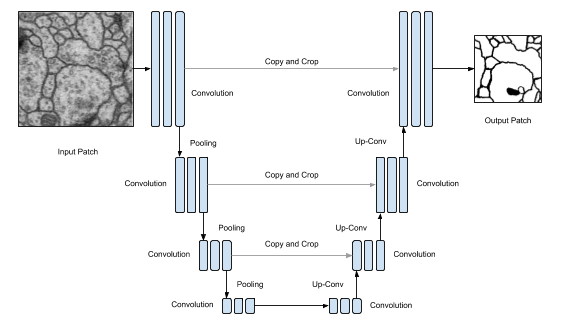
\includegraphics[width=\textwidth]{img/U_Net.png}
\caption[A prototypical U-Net]{A prototypical U-Net, with successive convolutional layers followed by pooling layers on the downward pass, and then successive convolutional layers followed by up-convolutions on the upward pass. Notice how the inputs to each convolution after an up-convolution also takes as input the output of the last convolution of the corresponding layer in the downward pass.}
\label{fig:u_net}
\end{figure}

U-Net style architectures closely resemble autoencoders, in that they compress a representation of an input using convolutions and poolings, and then decompress that representation using convolutions and up-convolutions.  However, instead of trying to predict a perfect reconstruction of the input, the U-Net architeture attempts to reconstruct boundaries/affinities for the input image. One key feature of U-Nets is the symetrical use of skip connections - for every convolutional layer on the compressive (downward) pass, the output of those convolutions is added to the input of corresponding convolutional layers on the decompressive (upward) pass. This serves to force the net to quickly learn a set of affinities that look like the input. Much like Standard Convolutional Networks, every pixel in the output patch of a U-Net architecture can be affected by pixels in a certain field of view in the original input - modifying this field of view can often modify the quality of the results. Empirically, the predictions of U-Net architectures tend to be significantly smoother than fully convolutional architectures (although they may not be more accurate). A prototypical U-Net can be seen in Figure \ref{fig:u_net}. Architectures that are primarily based on the U-Net style are the original U-Net (2 dimensional) and 3D U-Net (3 dimensional). SegNet also resembles the U-Net architecture, in drawing inspiration from the autoencoder paradigm.

\subsubsection{Residual Nets}

\begin{figure}
\centering
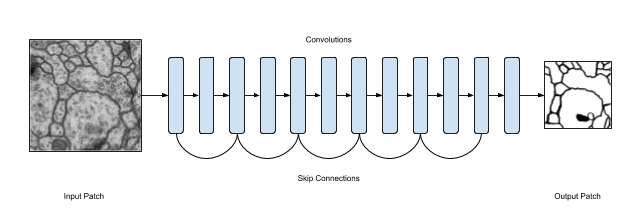
\includegraphics[width=\textwidth]{img/Residual_Network.png}
\caption[A prototypical Residual Net]{A prototypical Residual Net, which has a similar structure to the Fully Convolutional Network. The major difference is the skip connections - the residual connections - are added right before the nonlinearity but after a convolution. Residual connections can be added to other architectures to achieve some of the properties of this network.}
\label{fig:residual_net}
\end{figure}

Residual Networks draw on a similar idea as U-Net, in that convolutional layers should be able to directly influence layers that do not directly follow them in the architecture. As shown in Figure \ref{fig:residual_net}, Residual Nets add skip connections that jump over one (or more) sets of convolutions. Deeper nets are, in general, quite difficult to train, and the use of residual connections often increases the speed of training for deeper architectures.

\subsubsection{Flood-Filling Networks}
Flood-Filling Networks (FFNs) take a different approach to the prediction task. Rather than predict whether a pixel in the output is a boundary or not on a given input, FFNs are given an input patch and an x-y coordinate, and output a pixel mask for that patch that represents whether a pixel in the output is in the same body as the input x-y coordinate. If a particular object is sampled such that the output patches completely cover the object, a full segmentation of that object can be achieved (successive sample patches are chosen by a recurrent neural net (RNN)). Typically, this map is predicted with several convolutions, although architectures are varied. While we will not explore FFNs any further, as they are outside the scope of the research presented in this paper, they are noteworthy in that directly predict segmentation, rather than an intermediate (and thus require substantially less postprocessing than other menthods).


\subsubsection{Typical Errors}
The errors made by neural networks in the Image Transformation stage (and ultimately affect the accuracy of the resulting segmentation) tend to fall into several categories: split errors, merge errors, and incorrect object shaping. These errors are somewhat self-explanatory. Split errors occur when networks predict intermediates that, when converted into a segmentation, incorrectly split a body into two distinct segments when it should be one. Similarly, merge errors occur when two distinct objects are labeled as the same object. Incorrect object shaping occurs when the output of the network incorrectly predicts boundaries that may not necessarily cause merge or split errors, but simply predict boundaries that are too thick or otherwise encroach on the true shape of the object. These sorts of errors can be mitigated either by altering network architecture, or through postprocessing.

Important to note is the fact that the quality of the input data has a huge effect on the quality of the output data. While data augmentations during training can help networks compensate for misaligned data, generally inputs that are well-aligned will result in significantly better predictions than those that are poorly aligned. It is difficult to completely correct for this at the Image Transformation stage, which is why we stress the importance of the Preprocessing stage in preparing data well for segmentation.

\subsection{Postprocessing}
Once the EM stack data has been transformed into an intermediate form (i.e. boundaries/affinities, or segementation in the case of Flood-Filling Networks), postprocessing is often applied. Postprocessing can take on many forms, but often involve using the intermediate form to prepare a segmentation. Given a boundary/affinity map, there are many different ways to infer a segmentation of an image. However, we will discuss two methods that are used in the Seung Lab to process boundaries/affinities into segmentations.

\subsubsection{Watershed Transform}
The Watershed Transform is a standard computer vision algorithm for segmenting images. Given an affinity graph, the algorithm treats the values of affinities as energy values, which is analogous to the height of land in a geographical landscape. Since pixels that belong to the same body have high affinity, the topological high-points will be the bodies themselves, and the valleys will be the boundaries between bodies. The watershed variant used in the Seung Lab identifies the plateaus (representing distinct objects) and uses those identified plateaus to inform where to place basins for the classical watershed algorithm. The algorithm then floods basins based on a set of supplied parameters. This allows a distinct labeling of all pixels in the image, where pixels in the same basin are given the same label. All bodies that are too small to actually be distinct bodies are merged greedily. It is at this stage where merge/split errors often manifest, since two basins could be split or merged if there are discontinuities in an affinity boundary, or if non-cell-wall affinites are too high. Selecting appropriate parameters for this task is paramount in finding a good segmentation, and is typically performed empirically for a given dataset.

\subsubsection{Mean Affinity Agglomeration}
One way to mitigate some of the merge/split errors that arise from the Watershed Transform's intolerence of slightly imprecise affinities is to artificially heal the imperfections in boundaries that are generally correct. Mean Affinity Agglomeration (MAA) is one way to do this. MAA iterates over boundaries between segmented objects and greedily merges or splits them based on the mean affinity along the boundary. In this way, inconsistent boundaries predicted by the Image Transform stage can be healed.

\subsection{Segmentation/Downstream Processing}
Once postprocessing has occurred, the data is now in a completely segmented form. The segmentation can then be used for downstream tasks. Theoretical applications of segmentation include labeling different cells by their type, generating weighted directed graphs that represent connections between neurons, and determining characteristics of neurons in different types of tissue.